\begin{figure}[!htb]
  \centering
  \begin{subfigure}{0.08\textwidth}
    \centering
    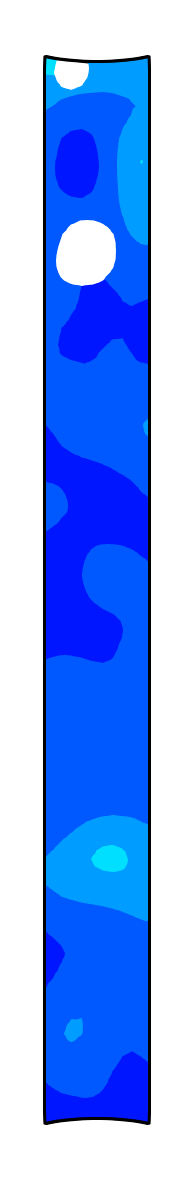
\includegraphics[width=\textwidth]{Chapter5/figures/spallation/ep_1}
  \end{subfigure}
  \begin{subfigure}{0.08\textwidth}
    \centering
    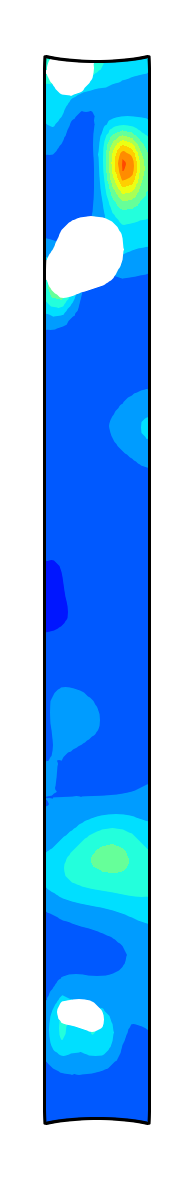
\includegraphics[width=\textwidth]{Chapter5/figures/spallation/ep_2}
  \end{subfigure}
  \begin{subfigure}{0.08\textwidth}
    \centering
    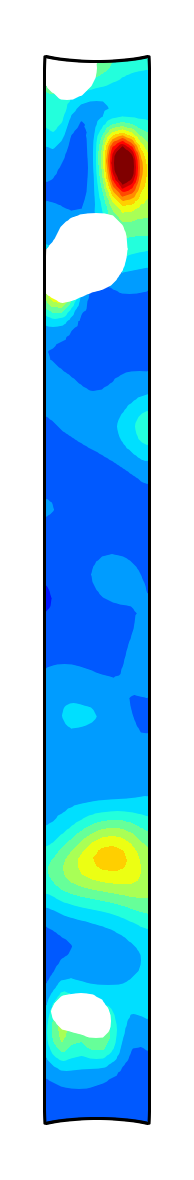
\includegraphics[width=\textwidth]{Chapter5/figures/spallation/ep_3}
  \end{subfigure}
  \begin{subfigure}{0.08\textwidth}
    \centering
    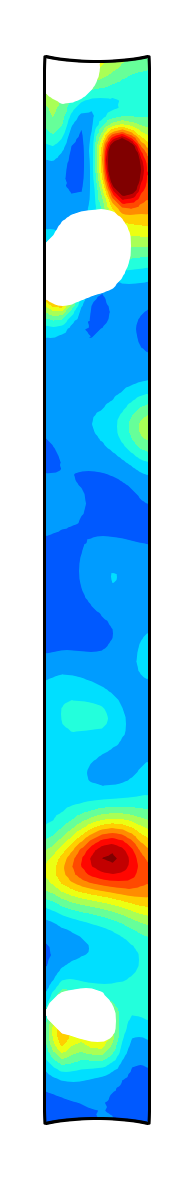
\includegraphics[width=\textwidth]{Chapter5/figures/spallation/ep_4}
  \end{subfigure}
  \begin{subfigure}{0.08\textwidth}
    \centering
    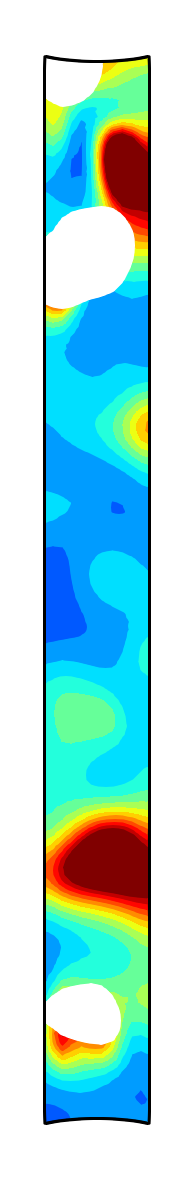
\includegraphics[width=\textwidth]{Chapter5/figures/spallation/ep_5}
  \end{subfigure}
  \begin{subfigure}{0.08\textwidth}
    \centering
    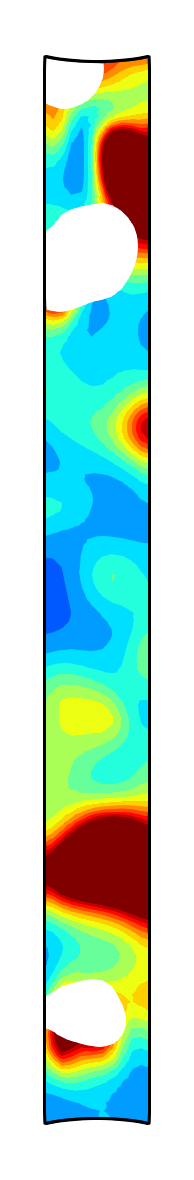
\includegraphics[width=\textwidth]{Chapter5/figures/spallation/ep_6}
  \end{subfigure}
  \begin{subfigure}{0.08\textwidth}
    \centering
    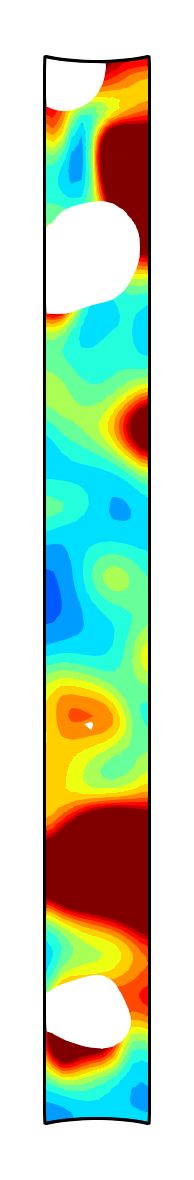
\includegraphics[width=\textwidth]{Chapter5/figures/spallation/ep_7}
  \end{subfigure}
  \begin{subfigure}{0.08\textwidth}
    \centering
    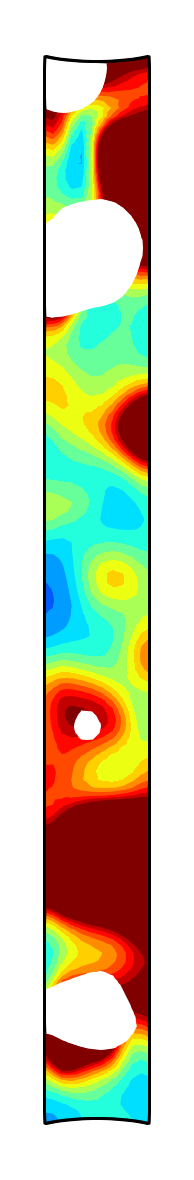
\includegraphics[width=\textwidth]{Chapter5/figures/spallation/ep_8}
  \end{subfigure}
  \begin{subfigure}{0.08\textwidth}
    \centering
    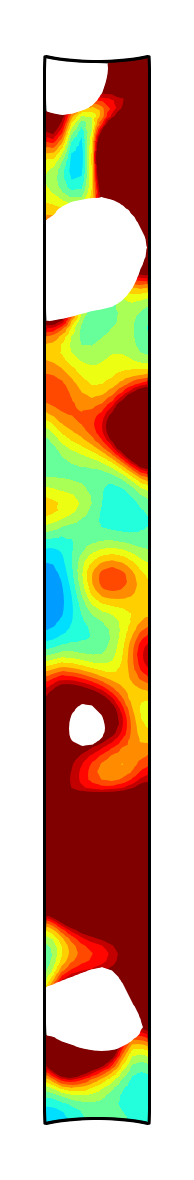
\includegraphics[width=\textwidth]{Chapter5/figures/spallation/ep_9}
  \end{subfigure}
  \begin{subfigure}{0.08\textwidth}
    \centering
    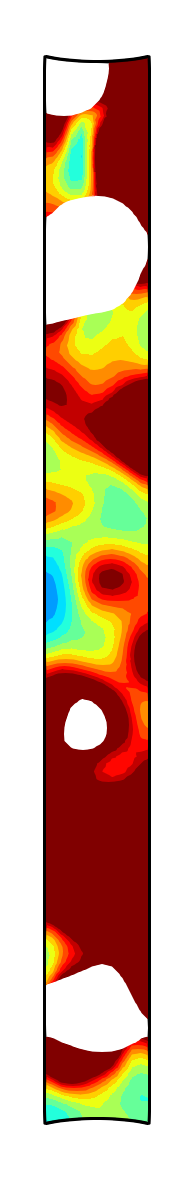
\includegraphics[width=\textwidth]{Chapter5/figures/spallation/ep_10}
  \end{subfigure}
  \begin{subfigure}{0.1\textwidth}
    \centering
    \caption*{$\ep$}
    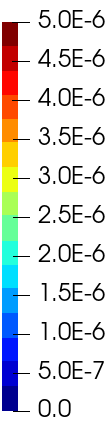
\includegraphics[width=\textwidth]{Chapter5/figures/spallation/colorbar_ep}
  \end{subfigure}
  \caption[The effective plastic strain right after each shut-down event.]{The effective plastic strain right after each shut-down event. The region within the contour of $d \leqslant 0.75$ is removed to visualize in-plane fracture.}
  \label{fig: Chapter5/spallation/animation_ep}
\end{figure}
